\section{Results}
\subsection{Performance Evaluation}
\begin{figure}[h]
    \centering
    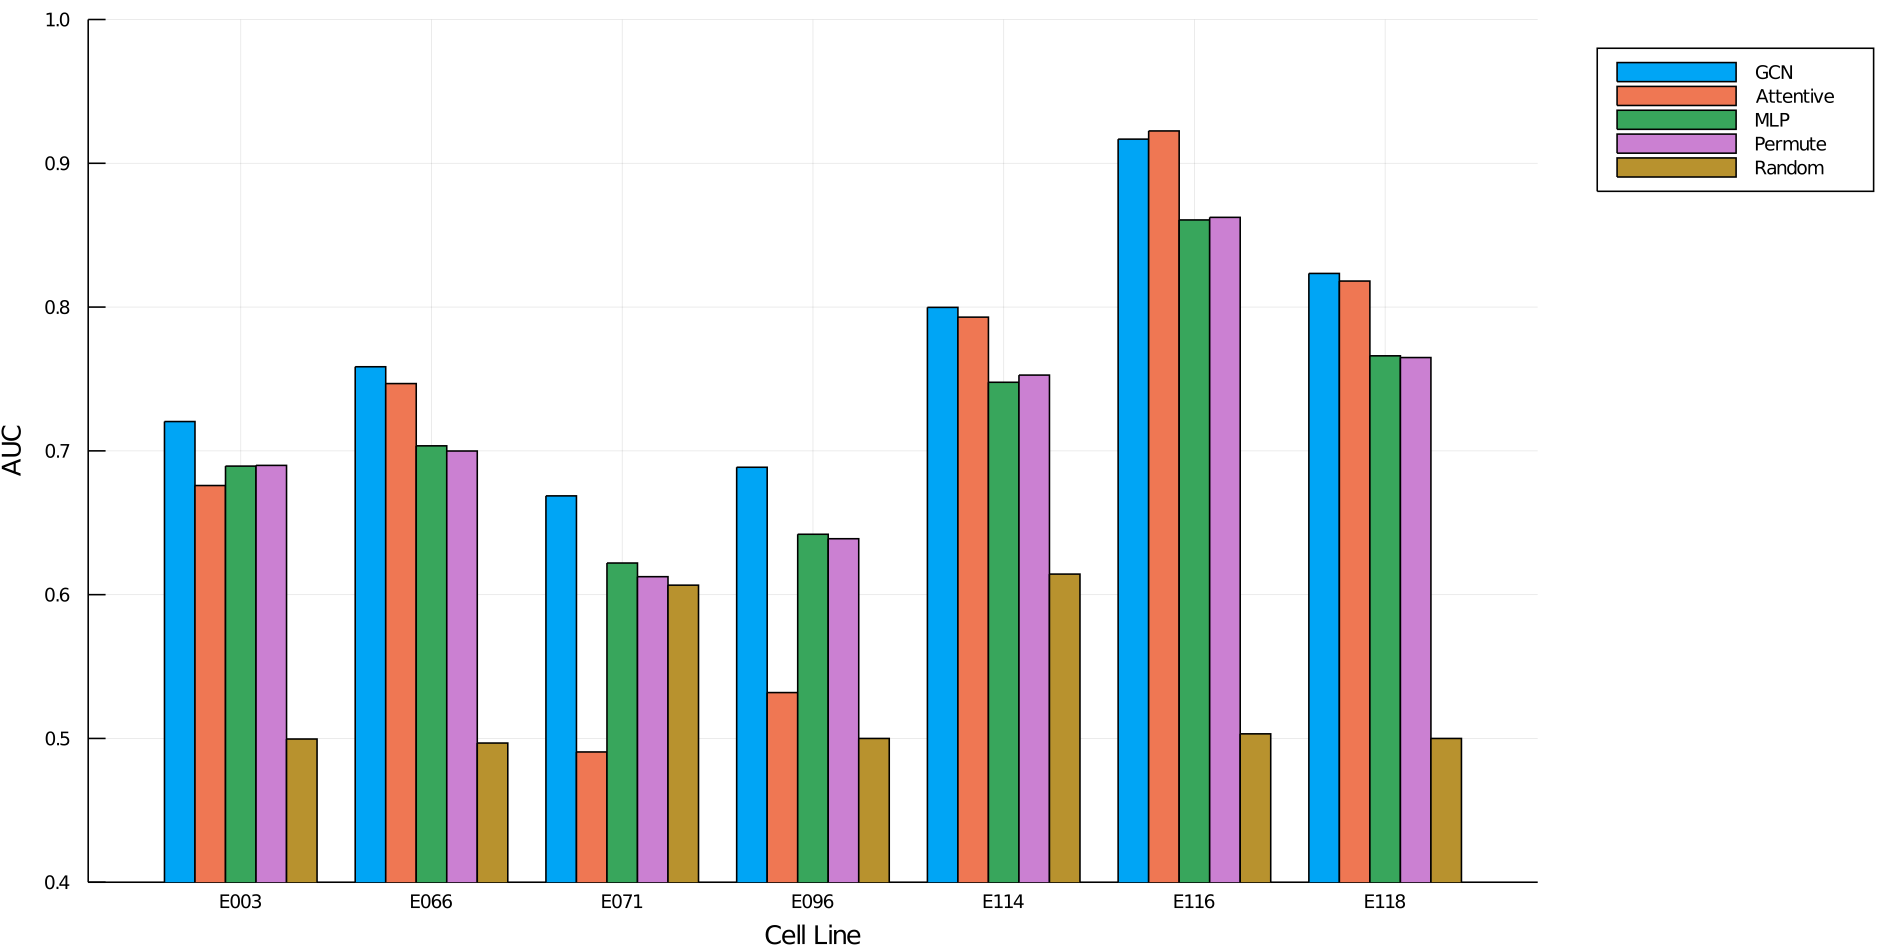
\includegraphics[width=\textwidth]{images/performance_bar.png}
    \begin{tabular}{l || c | c | c | c | c | c | c || r}
        & E003 & E066 & E071 & E096 & E114 & E116 & E118 & \emph{Average}\\ \hline 
        GCN & \textbf{0.7204} & \textbf{0.7585} & \textbf{0.6687} & \textbf{0.6886} & \textbf{0.7998} & 0.9168 & \textbf{0.8234} & \textbf{0.7655} \\
        Attentive & 0.6759 & 0.7468 & 0.4906 & 0.5319 & 0.7930 & \textbf{0.9225} & 0.8181 & 0.7113 \\
        MLP & 0.6894 & 0.7035 & 0.6220 & 0.6420 & 0.7477 & 0.8606 & 0.7661 & 0.7188 \\
        Permute & 0.6899 & 0.6999 & 0.6125 & 0.6389 & 0.7527 & 0.8624 & 0.7649 & 0.7094 \\
        Random & 0.4996 & 0.4968 & 0.6066 & 0.5000 & 0.6143 & 0.5032 & 0.5000 & 0.5229
    \end{tabular}
    \caption{AUC Performance Across Cell Lines and Baseline Methods}
    \label{figure:Figure1}
\end{figure}
The performance of the model was checked against four baselines across seven different cell lines and is summarized in Figure \ref{figure:Figure1}. \\\\
Quite clearly, the GCN model outperforms almost all of the other baseline methods, including the state of the art AttentiveChrome, across the cell lines. The only cell line where the GCN model was beaten was in the E116 cell line which was high performing across models. It is clear, though, that the GCN model shows great consistency and proves performance gains in lower performing cell lines such as E071. This is encapsulated in the average AUC performance metric across cell lines where the GCN model has a significantly higher average than all other models and in Figure \ref{figure:Figure1}. Note that AUC scores above are calculated using the weighted method to correct for any potential class imbalances in the datasets.
 